\documentclass[11pt,a4paper,fontset=fandol]{ctexart}
\usepackage[a4paper,margin=22mm,headheight=14pt]{geometry}
\usepackage{amsmath,amssymb}
\usepackage{booktabs,tabularx,longtable,multirow,threeparttable}
\usepackage{graphicx}
\usepackage{subcaption}
\usepackage{xcolor}
\usepackage{siunitx}
\usepackage{enumitem}
\usepackage{microtype}
\usepackage{fancyhdr}
\usepackage{hyperref}
\usepackage[nameinlink,noabbrev]{cleveref}
\usepackage{float}
\usepackage{placeins}

\definecolor{PAIBlue}{HTML}{3B6FB6}
\definecolor{PAITeal}{HTML}{2A9D8F}
\hypersetup{colorlinks=true,linkcolor=PAIBlue,citecolor=PAITeal,urlcolor=PAIBlue}
\graphicspath{{figures/}}
\captionsetup{font=small,labelfont=bf,justification=justified,singlelinecheck=false}
\setlist{nosep,leftmargin=1.7em}
\sisetup{group-separator={,},group-minimum-digits=4,detect-all}
\emergencystretch=2em
\crefname{figure}{图}{图}
\Crefname{figure}{图}{图}
\crefname{table}{表}{表}
\Crefname{table}{表}{表}
\crefname{section}{第}{节}
\Crefname{section}{第}{节}

\pagestyle{fancy}
\fancyhf{}
\lhead{工业世界模型项目报告}
\rhead{世界模型与策略优化}
\cfoot{\thepage}

\title{面向工业过程控制的世界模型：\\状态演化建模、策略优化与 NeoRL 仿真验证}
\author{}
\date{\today}

\begin{document}
\maketitle
\begin{abstract}
本文基于 NeoRL Industrial Benchmark 构建面向工业过程控制的世界模型（World Model）与策略优化流程。针对100、1000和10000条训练轨迹三种数据规模，比较 MLP、GRU、LSTM、Transformer-2L 和 Transformer-4L 的状态预测能力，并结合单步预测与多步递归预测评价模型；随后使用冻结的世界模型比较 CEM、iCEM、MPPI 和 MB-PPO，在 NeoRL 仿真环境中进行1000步长期控制验证。小规模数据下 GRU 的综合预测误差最低，中、大规模数据下 Transformer-2L 更优。最终 M100 采用 GRU+CEM，M1000 和 M10000 采用 Transformer-2L+MPPI，1000步累计奖励分别为 $-274{,}181$、$-220{,}129$ 和 $-223{,}876$，相对行为克隆（BC）基础策略分别提高14,229、68,282和64,535。所构建的世界模型能够支持后续策略优化，并在当前基准中改善长期控制效果。
\end{abstract}
\clearpage
\tableofcontents
\clearpage

\section{项目概述}
\label{sec:intro}
工业过程通常具有长时滞、变量耦合以及直接试错成本高等特点。仅依靠历史轨迹训练策略，难以在执行前回答“某个控制动作将使设备状态如何演化”；直接在真实设备上反复搜索动作则可能带来能耗、磨损和安全风险。本项目从已有工业轨迹学习可递归预测未来状态的世界模型，再利用冻结模型进行动作序列规划或策略学习，最后在 NeoRL 仿真环境中验证长期控制效果。

整体技术路线见\cref{fig:framework}。历史状态序列和动作首先用于训练世界模型；模型通过单步预测和多步递归预测评价后被冻结，分别支持基于模型的规划方法 CEM、iCEM、MPPI，以及基于模型的强化学习方法 MB-PPO。经过优化的策略最终在 NeoRL 仿真环境中执行，以1000步累计奖励衡量长期控制效果。

\begin{figure}[H]
  \centering
  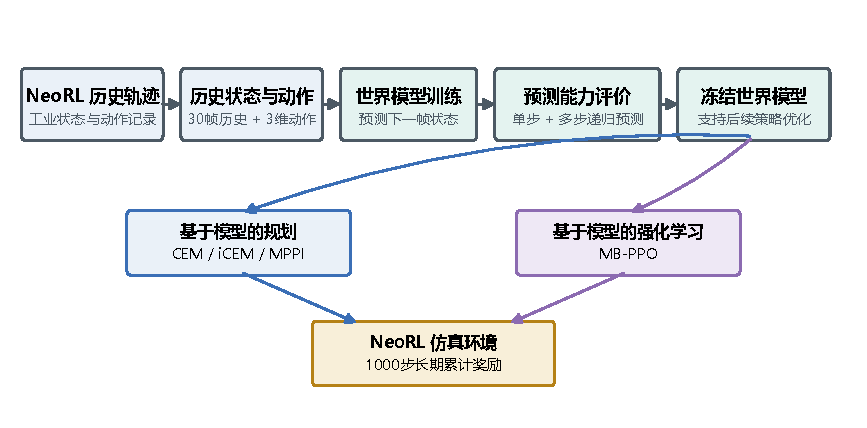
\includegraphics[width=\textwidth]{fig1_framework.pdf}
  \caption{\textbf{项目整体技术路线。} NeoRL 历史轨迹被整理为历史状态序列与连续动作，用于训练下一状态预测模型。世界模型经过单步与多步预测评价后被冻结，并分别服务于基于模型的规划和基于模型的强化学习；优化后的控制策略在 NeoRL 仿真环境中验证长期累计奖励。}
  \label{fig:framework}
\end{figure}

本项目比较五类世界模型、三种规划方法和一种基于模型的强化学习方法。最终在 M100 上选择 GRU+CEM，在 M1000 与 M10000 上选择 Transformer-2L+MPPI。正文依次介绍状态与奖励定义、世界模型构建与评价、策略优化方法、仿真实验结果，以及这些结果对工业部署的启示。


\section{问题定义与数据}
\label{sec:problem}
\subsection{State, action and transition}

NeoRL Industrial Benchmark中的观测为180维向量，可重排为30个历史帧，每帧包含6个物理变量：setpoint、velocity、gain、shift、fatigue和consumption。动作 $a_t\in[-1,1]^3$ 是三维连续控制量。令单帧为 $x_t\in\mathbb{R}^{6}$，历史窗口为 $x_{t-29:t}$，World Model学习
\begin{equation}
  \left(x_{t-29:t},a_t\right)\longmapsto \hat{x}_{t+1}.
\end{equation}
预测下一帧后，将 $\hat{x}_{t+1}$ 放入窗口最前端并移除最旧帧，得到下一次递归预测所需的180维状态。这个滑动窗口使所有架构具有一致输入输出：$[B,30,6]$ history与$[B,3]$ action映射到$[B,6]$ next frame。

\subsection{Reward and evaluation roles}

NeoRL的classic industrial reward为
\begin{equation}
  r_{t+1}=-\left(3\,\mathrm{fatigue}_{t+1}+\mathrm{consumption}_{t+1}\right).
\end{equation}
因此，降低设备疲劳和资源消耗会使reward变得更高（更不负）。本文报告1000步episode cumulative reward。需要强调的是，simulator reward只用于策略优化与最终控制评价，绝不参与World Model checkpoint或架构选择。

\subsection{Original Behavior reference}

原始行为数据参考值（Original Behavior）按如下方式定义：NeoRL数据集中的历史轨迹由原始行为策略采集。由于公开数据未提供可直接重新部署该采集策略的策略权重，本文统计数据集中已有轨迹的累计奖励作为原始行为水平参考；BC及世界模型优化策略则统一部署到NeoRL simulator中评估。因此Original Behavior用于描述原始数据行为水平，不与在线策略做严格的同seed配对统计。该区分也符合NeoRL强调数据分布、行为策略和部署验证应被谨慎区分的初衷\cite{qin2022neorl}。

三个数据规模M100、M1000与M10000分别提供不同数量级的历史轨迹。跨规模比较不以raw epoch数判断训练充分性，因为不同规模的一轮训练对应不同样本数量；报告只比较统一common-validation上的最终预测指标。


\section{世界模型设计}
\label{sec:wm_design}
\subsection{Compared architectures}

本文比较五类正式架构。MLP把完整历史窗口展平后进行静态非线性映射；GRU和LSTM通过递归隐状态提取时间依赖，其中GRU使用较简化的门控结构，LSTM使用显式记忆单元；Transformer-2L和Transformer-4L通过self-attention直接建模30帧之间的依赖\cite{vaswani2017attention}。Transformer深度实验只改变层数2到4，$d_{model}$、head数、FFN宽度和dropout保持不变。


\begin{table}[H]
\centering
\caption{世界模型架构。参数量不随数据规模改变。}
\label{tab:architectures}
\small
\begin{tabularx}{\textwidth}{lXXr}
\toprule
模型架构 & 时间信息建模方式 & 主要配置 & 参数量 \\
\midrule
MLP & 无显式时序递归 & 2$\times$256，dropout 0.1 & 114,438 \\
GRU & 门控递归状态 & 2层，隐状态128，动作分支64 & 177,030 \\
LSTM & 带记忆单元的递归状态 & 2层，隐状态128，动作分支64 & 227,462 \\
Transformer-2L & 自注意力历史编码 & $d=64$，4头，FFN 128，2层 & 91,142 \\
Transformer-4L & 自注意力历史编码 & $d=64$，4头，FFN 128，4层 & 158,086 \\
\bottomrule
\end{tabularx}
\end{table}


所有模型共享数据划分、normalization、optimizer、trainer、checkpoint规则和evaluation protocol。不同架构的参数量约为9万至23万，规模足够轻量，便于突出时序归纳偏置而不是单纯扩大容量。

\subsection{Validation metrics and selection}

NRMSE使用固定common-validation目标标准差归一化，使不同架构和数据规模可以在同一口径下比较。评价包括one-step NRMSE，以及使用真实记录动作但递归更新预测状态的H1、H5、H10、H20和H50 NRMSE。Per-variable error用于判断某个整体指标是否被特定物理变量主导。

模型选择只使用validation dynamics：
\begin{enumerate}
  \item 找到该数据规模下最低的one-step NRMSE；
  \item 保留满足 $\mathrm{one\mbox{-}step}\leq1.10\times\mathrm{best\ one\mbox{-}step}$ 的候选；
  \item 在候选中最小化 $\mathrm{mean}(\mathrm{H5},\mathrm{H10},\mathrm{H20})$；
  \item H50仅作为长期rollout稳定性诊断。
\end{enumerate}
这个规则先排除单步明显不合格的模型，再选择短中期递归预测最稳定者。任何CEM、iCEM、MPPI或MB-PPO simulator reward都不进入上述流程。


\section{世界模型实验结果}
\label{sec:wm_exp}
\subsection{Architecture $\times$ Data Scale}

正式比较包含5种架构与3个数据规模，共15组World Model。\Cref{fig:wm_heatmaps}用两个annotated heatmap分别回答单步与多步问题；每个单元格都来自同一common-validation protocol，橙色边框表示最终validation选择。

\begin{figure}[H]
  \centering
  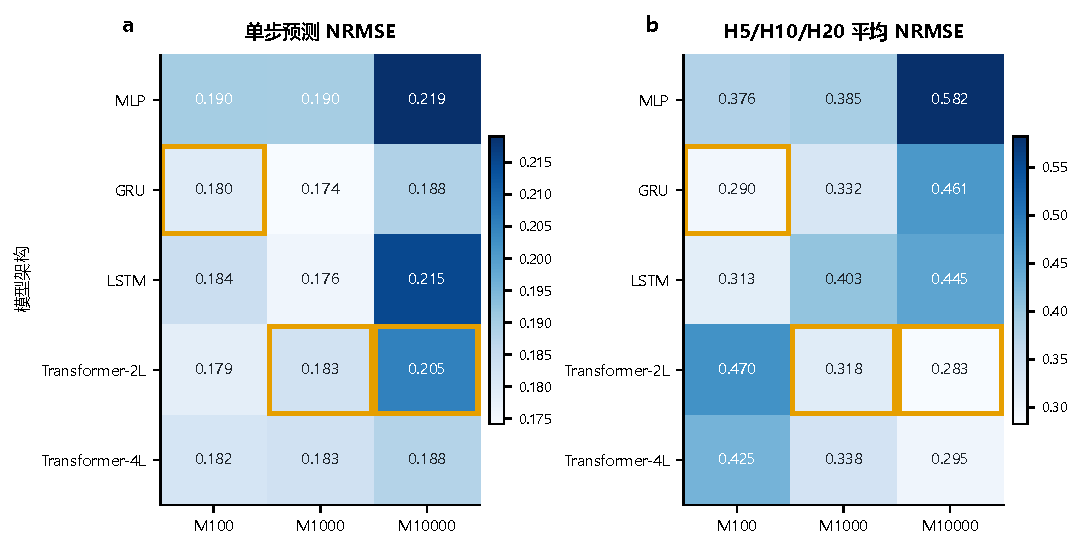
\includegraphics[width=\textwidth]{fig2_world_model_heatmaps.pdf}
  \caption{\textbf{Architecture and dataset scale jointly shape dynamics accuracy.} \textbf{a}, one-step NRMSE。\textbf{b}, mean NRMSE at H5/H10/H20。数值越低越好，橙色边框表示validation-only规则选出的模型。M100偏好GRU；M1000和M10000偏好Transformer-2L。两张heatmap的排序并不完全一致，说明单步指标不能替代递归评价。}
  \label{fig:wm_heatmaps}
\end{figure}

M100中，GRU在合格one-step候选里取得最低的短中期综合误差；M1000与M10000则由Transformer-2L胜出。该结果不支持``某一架构永远最好''，而是说明时序归纳偏置与数据规模存在交互。尤其是M10000中MLP并未因数据更多而自动获得更好结果，提示数据覆盖、优化预算和架构表达能力需要共同考虑。


\begin{table}[H]
\centering
\caption{统一验证选出的世界模型。H50 仅用于长期稳定性诊断。}
\label{tab:selected_wm}
\small
\begin{tabular}{lllrrrrr}
\toprule
数据规模 & 模型架构 & 选定轮次 & 单步 & H5 & H10 & H20 & H50 \\
\midrule
M100 & GRU & 35 & 0.180 & 0.223 & 0.273 & 0.374 & 0.649 \\
M1000 & Transformer-2L & 20 & 0.183 & 0.243 & 0.305 & 0.405 & 0.774 \\
M10000 & Transformer-2L & 4 & 0.205 & 0.258 & 0.298 & 0.293 & 0.510 \\
\bottomrule
\end{tabular}
\end{table}


\subsection{One-step and multi-step prediction}

One-step只评价在真实历史状态条件下预测下一帧；实际规划会把预测值重新输入模型，因此误差会改变后续输入分布。\Cref{fig:multistep}固定M1000并展示五个正式architecture checkpoint在五个真实评价horizon上的结果，不做插值或平滑。

\begin{figure}[H]
  \centering
  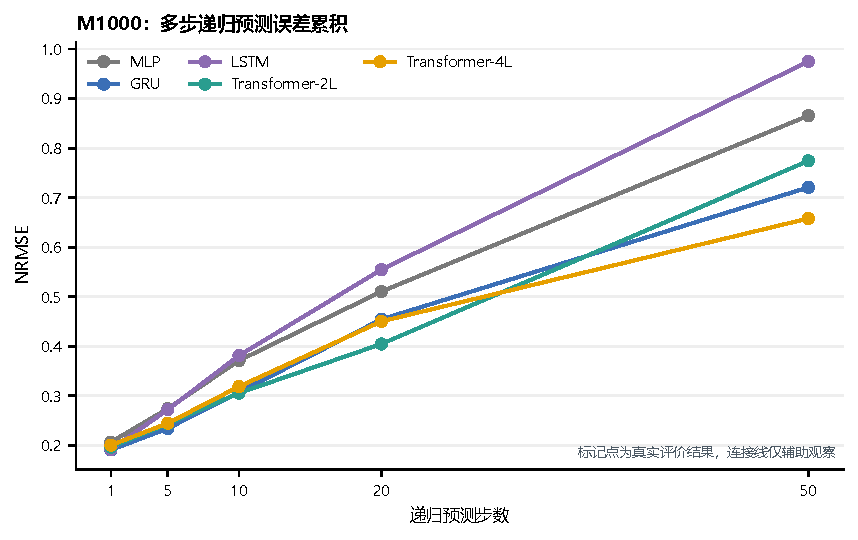
\includegraphics[width=0.92\textwidth]{fig3_multistep_error.pdf}
  \caption{\textbf{Recursive prediction error accumulation at M1000.} 五个marker对应H1、H5、H10、H20和H50的真实评价点，连接线只辅助阅读。尽管H1均接近0.2，不同架构在H20--H50明显分离；Transformer-2L在H5--H20综合最好，而Transformer-4L的H50更低。}
  \label{fig:multistep}
\end{figure}

Per-variable结果进一步说明overall NRMSE并不等同于每个工业变量都同样准确。Setpoint在该benchmark中较稳定，而velocity、shift、fatigue和consumption的误差演化不同。\Cref{tab:per_variable}列出M1000 Transformer-2L的代表性变量级结果。


\begin{table}[H]
\centering
\caption{M1000 Transformer-2L 的变量级 NRMSE。不同物理变量的误差累积速度明显不同。}
\label{tab:per_variable}
\small
\begin{tabular}{lrrr}
\toprule
物理变量 & 单步 & H20 & H50 \\
\midrule
设定值 & 0.000 & 0.000 & 0.000 \\
速度 & 0.029 & 0.310 & 0.704 \\
增益 & 0.018 & 0.292 & 0.012 \\
偏移 & 0.036 & 0.670 & 1.498 \\
疲劳度 & 0.378 & 0.432 & 0.510 \\
能耗 & 0.234 & 0.406 & 0.773 \\
\bottomrule
\end{tabular}
\end{table}


\Cref{fig:rollout}提供一条直观轨迹。为避免选择最好看的样本，先在101个确定性validation起点上计算H50误差，再选择最接近中位误差的起点；动作来自记录轨迹，只有状态递归使用模型预测。

\begin{figure}[H]
  \centering
  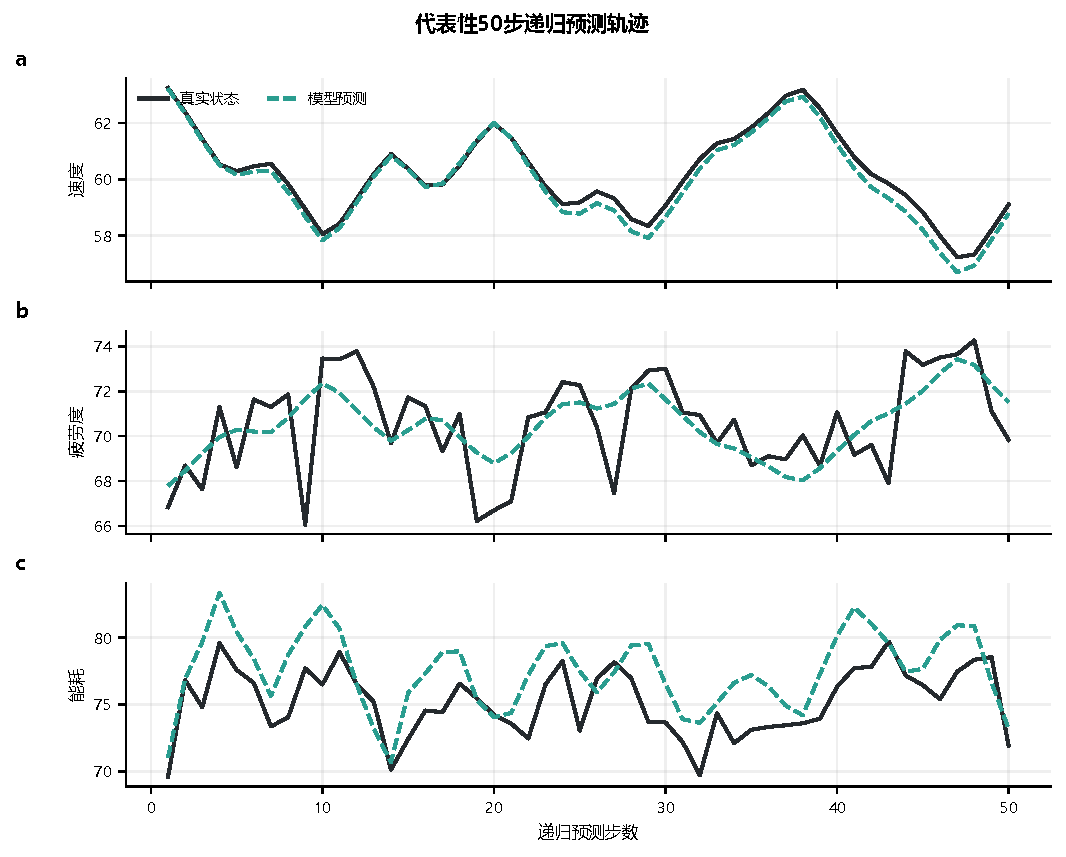
\includegraphics[width=0.94\textwidth]{fig4_representative_rollout.pdf}
  \caption{\textbf{Representative H50 recursive rollout.} \textbf{a--c}, velocity、fatigue与consumption的ground truth和prediction。该轨迹按预先规定的中位误差规则选择，不代表最好或最差情况。短期趋势可以跟随真实状态，但变量级偏差会以不同方式累积；总体结论仍应以全体validation起点的NRMSE为准。}
  \label{fig:rollout}
\end{figure}

\subsection{Transformer depth ablation}


\begin{table}[H]
\centering
\caption{Transformer 深度消融。单元格为单步 NRMSE / H5、H10、H20 平均 NRMSE；差值为4L减2L，负值表示4L更优。}
\label{tab:depth}
\small
\begin{tabular}{lccc}
\toprule
数据规模 & Transformer-2L & Transformer-4L & 差值 \\
\midrule
M100 & 0.179 / 0.470 & 0.182 / 0.425 & +0.003 / -0.044 \\
M1000 & 0.183 / 0.318 & 0.183 / 0.338 & +0.000 / +0.020 \\
M10000 & 0.205 / 0.283 & 0.188 / 0.295 & -0.017 / +0.012 \\
\bottomrule
\end{tabular}
\end{table}


M100中4L改善了多步综合误差但单步略差；M1000中4L的H50更低，但H5--H20综合反而更高；M10000中4L单步更好，却在H20与综合指标上落后2L。由此不能得到``层数增加会随数据规模稳定增强''的结论，也没有证据支持继续扩大到6L。这里的重点是严格控制变量后的深度效应，而不是把不同训练预算或旧结果混入比较。


\section{基于世界模型的策略优化}
\label{sec:strategy}
\subsection{Model-Based Planning}

Model-Based Planning在每个simulator step利用冻结World Model评估候选动作序列，只执行最前面的动作，然后根据新观测重新规划。

\begin{itemize}
  \item \textbf{CEM}：从参数化动作分布采样，保留高回报elite序列，并迭代更新均值和方差。它是一种不依赖梯度的轨迹优化方法。
  \item \textbf{iCEM}：在CEM基础上加入temporal colored noise、elite reuse、previous-solution shift和population decay等机制，以更少样本复用过去规划信息\cite{pinneri2021icem}。
  \item \textbf{MPPI}：基于路径积分和importance weighting，对大量带噪动作序列按预测cost赋权，再更新控制序列\cite{williams2017mppi}。通俗地说，它不是只保留少数elite，而是让更优样本获得更高权重。
\end{itemize}

三种方法均使用H=10作为主horizon，并遵守$[-1,1]^3$动作约束。World Model全程冻结，规划结果不能反向修改模型。

\subsection{Model-Based Reinforcement Learning}

MB-PPO在冻结World Model中生成imagined rollout，再用PPO的clipped surrogate objective更新actor和value network\cite{schulman2017ppo}。与每一步都在线搜索的planner不同，MB-PPO把模型中的优化结果压缩到一个可快速推理的policy中。

Behavior KL约束度量当前policy与BC所代表的离线行为分布之间的偏离，并把该偏离加入训练目标。其通俗含义是：即使World Model认为某个数据分布外动作非常有利，policy也不能毫无代价地远离历史行为。\Cref{fig:kl_ablation}使用相同M1000 GRU World Model、初始化、rollout和PPO协议，只改变是否加入behavior KL。

\begin{figure}[H]
  \centering
  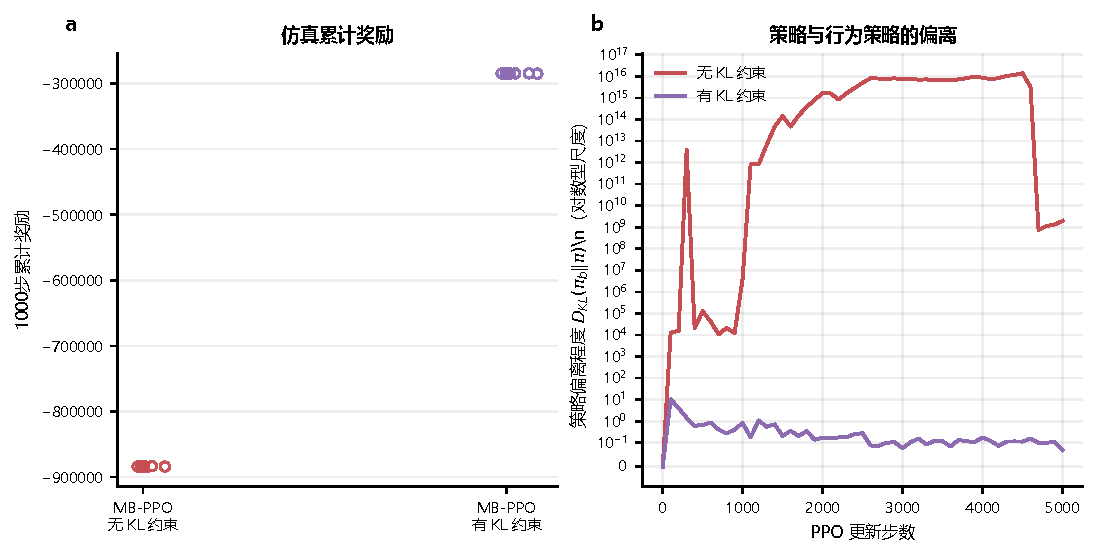
\includegraphics[width=\textwidth]{fig8_mbppo_kl_ablation.pdf}
  \caption{\textbf{Behavior-KL ablation for MB-PPO.} \textbf{a}, 相同五个development seeds上的simulator return；空心点为单seed，实心点及误差条为mean $\pm$ population SD。\textbf{b}, 训练期间相对BC的behavior KL。去除KL后policy divergence扩大，平均return由约$-2.85\times10^5$降至$-8.84\times10^5$。该消融支持behavior constraint能抑制当前设置中的model exploitation，但不确定最佳KL系数。}
  \label{fig:kl_ablation}
\end{figure}


\section{NeoRL 仿真验证}
\label{sec:evaluation}
\subsection{Strategy comparison across data scales}

每个数据规模固定由dynamics validation选择出的同一个World Model，再比较CEM、iCEM、MPPI与MB-PPO。所有方法使用相同development seeds 42--46、相同1000步episode和相同reward definition。因此，\cref{fig:strategy_matrix,tab:strategy_matrix}中的差异主要来自strategy与固定World Model之间的交互，而不是更换模型或seed。

\begin{figure}[H]
  \centering
  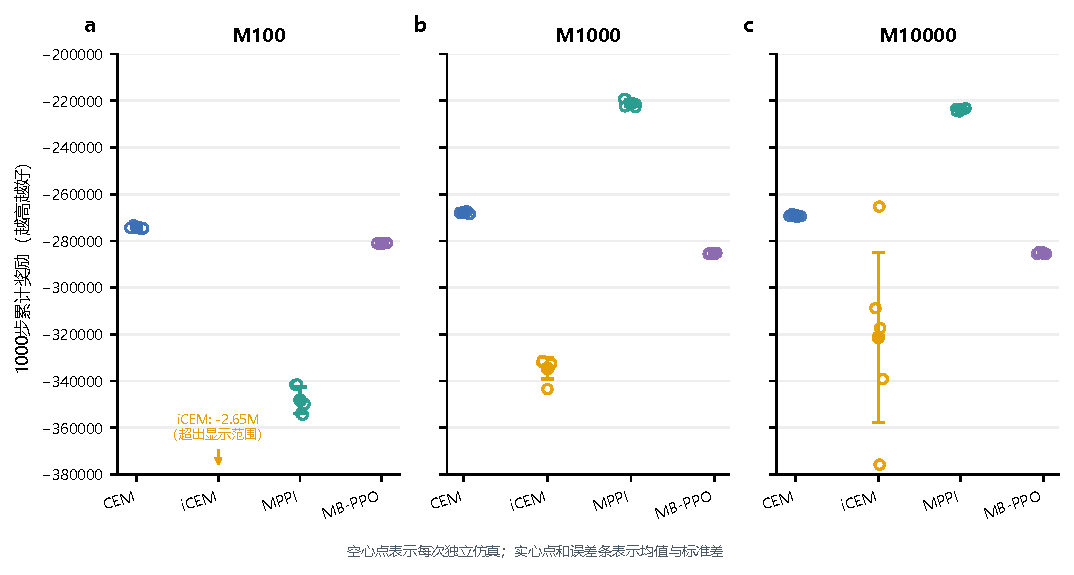
\includegraphics[width=\textwidth]{fig5_strategy_comparison.pdf}
  \caption{\textbf{Development strategy comparison across data scales.} \textbf{a--c}, M100、M1000和M10000。空心点为seeds 42--46，实心点及误差条为mean $\pm$ population SD。M100 iCEM明显超出主轴范围，因此在inset中保留全部五个seed。CEM在M100最高；MPPI在M1000和M10000最高。}
  \label{fig:strategy_matrix}
\end{figure}


\begin{table}[H]
\centering
\caption{Development strategy matrix (seeds 42--46). 数值为 episode cumulative reward 的 mean $\pm$ population SD，越高越好。}
\label{tab:strategy_matrix}
\scriptsize
\resizebox{\textwidth}{!}{%
\begin{tabular}{lrrrr}
\toprule
Dataset & CEM & iCEM & MPPI & MB-PPO \\
\midrule
M100 & -274,238 $\pm$ 588 & -2,646,910 $\pm$ 4,581 & -348,211 $\pm$ 5,687 & -281,009 $\pm$ 131 \\
M1000 & -267,826 $\pm$ 407 & -334,597 $\pm$ 4,503 & -221,072 $\pm$ 1,475 & -285,326 $\pm$ 158 \\
M10000 & -269,218 $\pm$ 411 & -321,264 $\pm$ 36,310 & -223,774 $\pm$ 578 & -285,217 $\pm$ 283 \\
\bottomrule
\end{tabular}}
\end{table}


M100上的iCEM和MPPI均明显落后，尤其iCEM出现一致的极低真实回报；相同算法通过了已知dynamics和cost上的deterministic optimization test，因此这里更合理的解释是弱World Model与optimizer之间发生model exploitation，而不是直接断言算法不适合Industrial Benchmark。M1000和M10000中MPPI的提升说明World Model质量是重要瓶颈。

\subsection{World Model $\times$ Strategy controlled ablation}

M1000进一步完成两组控制变量实验：第一组固定MPPI配置，仅改变五种World Model；第二组固定MB-PPO训练协议，仅改变World Model。该实验研究dynamics prediction ranking与downstream control ranking是否完全一致，不用于反向修改validation-only模型选择。

\begin{figure}[H]
  \centering
  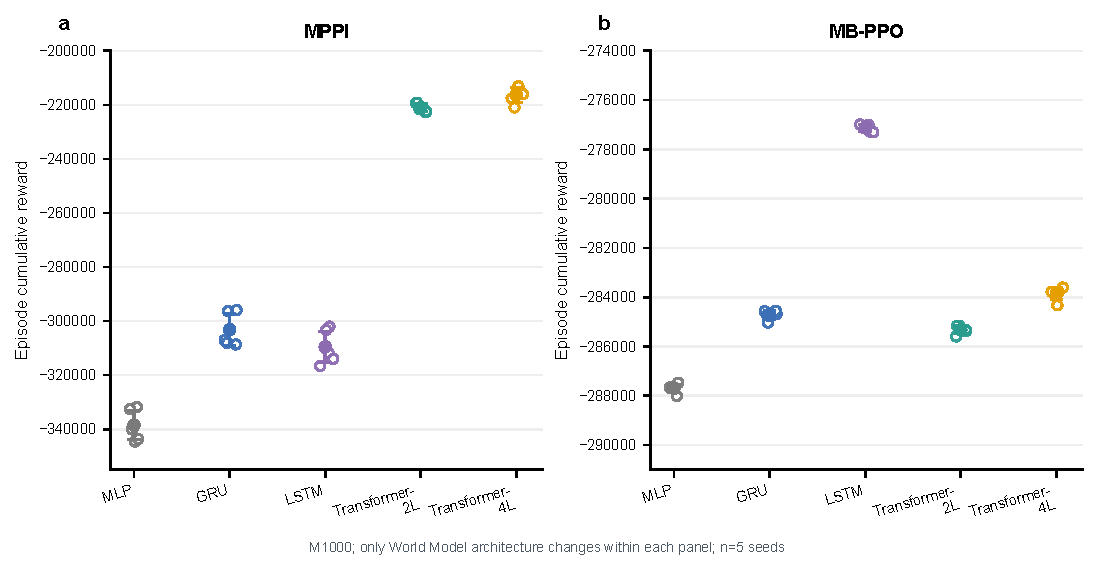
\includegraphics[width=\textwidth]{fig6_world_model_strategy_cross.pdf}
  \caption{\textbf{World Model architecture affects planning and learned policies differently.} \textbf{a}, 固定MPPI时五种World Model的development return。\textbf{b}, 固定MB-PPO protocol时的结果。每组$n=5$ seeds，点和误差条分别表示individual seed与mean $\pm$ population SD。MPPI在Transformer-4L上最高，而MB-PPO在LSTM上最高；dynamics validation最优仍为Transformer-2L。}
  \label{fig:cross}
\end{figure}

\subsection{Final simulator evaluation}

所有模型、strategy和设置冻结后，seeds 100--109才首次用于最终评价。最终系统按development结果确定：M100采用GRU+CEM，M1000与M10000采用Transformer-2L+MPPI。\Cref{fig:final,tab:final}同时展示原始行为数据参考值、BC与三个最终系统。

\begin{figure}[H]
  \centering
  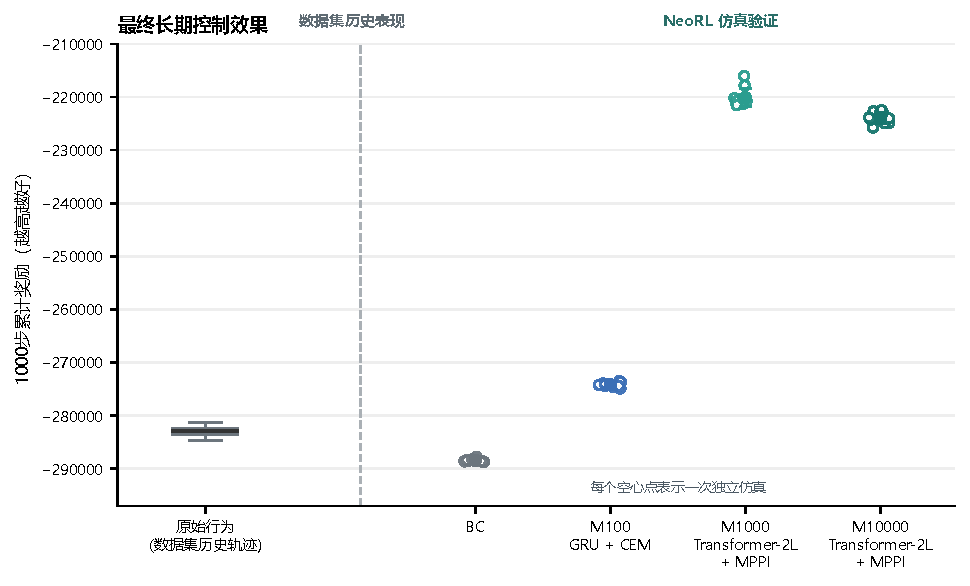
\includegraphics[width=\textwidth]{fig7_final_simulator.pdf}
  \caption{\textbf{Final NeoRL simulator results on untouched seeds.} Original Behavior以灰色box表示NeoRL数据集1000条已有轨迹的累计奖励分布，属于unpaired dataset-trajectory reference。其余方法均部署到NeoRL simulator；空心点为seeds 100--109，实心点及误差条为mean $\pm$ population SD。三个最终系统在十个seed上均优于BC。}
  \label{fig:final}
\end{figure}


\begin{table}[H]
\centering
\caption{Final NeoRL evaluation. Online systems use untouched seeds 100--109. Original Behavior来自数据集已有轨迹，不是同seed在线部署。}
\label{tab:final}
\scriptsize
\resizebox{\textwidth}{!}{%
\begin{tabular}{llrrr}
\toprule
Method/System & Evaluation source & Episode return & $\Delta$ vs BC & Win rate \\
\midrule
原始行为数据参考值（Original Behavior） & NeoRL dataset trajectories & -282,885 $\pm$ 1,197 & -- & -- \\
BC & NeoRL simulator & -288,411 $\pm$ 267 & 0 & -- \\
M100: GRU + CEM & NeoRL simulator & -274,181 $\pm$ 396 & +14,229 & 100\% \\
M1000: Transformer-2L + MPPI & NeoRL simulator & -220,129 $\pm$ 1,699 & +68,282 & 100\% \\
M10000: Transformer-2L + MPPI & NeoRL simulator & -223,876 $\pm$ 1,033 & +64,535 & 100\% \\
\bottomrule
\end{tabular}}
\end{table}


最终M100、M1000和M10000系统相对BC的平均提升分别为14,229、68,282和64,535，win rate均为100\%。这直接回答了Task 3：在当前NeoRL Industrial Benchmark设置中，经过严格模型选择和策略冻结的World-Model-based optimization能够提高长期cumulative reward。


\section{实验观察与讨论}
\label{sec:discussion}
\subsection{单步准确率不足以评价长期预测能力}

单步预测的输入始终来自真实历史，而规划和想象轨迹会递归使用模型自己的预测。M1000 中多个模型的单步 NRMSE 很接近，但 H20 和 H50 差距明显；单步误差最低的模型也不一定具有最低的 H5--H20 综合误差。该结果表明，面向控制的世界模型需要联合评价单步预测和多步递归预测，不能只依据单步损失决定部署模型。

\subsection{预测精度与控制效果并不完全一致}

M1000 控制变量实验中，统一预测评价选择 Transformer-2L；MPPI 在 Transformer-4L 上取得更高的策略比较阶段回报，MB-PPO 则在 LSTM 上表现更好。这一现象提示，通用预测误差与下游控制效果可能并不完全一致，不同策略也可能对不同类型的模型误差具有不同敏感性。该结论仅是当前五种架构、两类策略和一个数据规模上的实验观察，不应上升为普遍规律，也不用于反向修改世界模型选择。

\subsection{世界模型误差可能被策略优化放大}

M100 的结果显示，更复杂或采样更积极的优化器并不一定更可靠。规划器可能找到世界模型预测回报很高、但真实仿真表现较差的动作区域；当训练数据覆盖不足时，这类动作可能位于模型不可信的区域。因此，基于模型的控制不仅要优化预测回报，还需要判断候选动作是否受到历史数据支持。

\subsection{数据增加不一定带来单调的控制收益}

从 M100 到 M1000，最终累计奖励明显提高；从 M1000 到 M10000 则没有继续单调提高，M1000+MPPI 的最终平均回报略高。该结果可能与数据覆盖范围、模型架构、训练预算结构以及规划器对局部误差的敏感性共同有关。现有实验只能说明更多数据没有自动转化为更高控制回报，不能把差异唯一归因于某一个因素。

\subsection{模型架构与数据规模存在交互}

M100 中 GRU 取得更低的综合预测误差，提示递归结构在当前小数据设置中具有一定优势；M1000 和 M10000 中轻量的 Transformer-2L 更优；Transformer-4L 没有稳定获得进一步收益。因此，架构选择需要结合数据规模、递归预测长度和后续策略共同考虑，而不应预设 Transformer 或循环网络必然获胜。


\section{工业应用与部署思考}
\label{sec:industry}
\subsection{Potential industrial applications}

World Model能够在不直接扰动设备的情况下回答``如果改变控制量，未来状态可能如何演化''。潜在用途包括工艺参数优化、能耗与设备疲劳联合控制、future-state prediction、what-if control simulation、数字孪生、控制策略预验证、异常工况决策辅助，以及生产目标与设备状态的联合优化。对于复杂生产线，它还可以作为operator的决策支持工具，在执行动作前展示多种候选方案的预测后果。

\subsection{Deployment risks and safeguards}

真实工业数据比benchmark更复杂。Sensor noise、missing measurement、异常值和时间同步误差会直接污染30帧历史窗口；equipment aging、maintenance、生产配方和工况变化会造成dynamics drift；停机、故障与极端负载往往在offline data中极少出现，使模型在最重要的安全区域反而最不确定。部署前必须显式评估offline data coverage和out-of-distribution (OOD) operating conditions，而不能假设训练集大小足以代表所有未来状态。

控制层还必须处理hard safety constraints、actuator rate/position limits、多目标权衡和operator intervention。例如，疲劳与能耗的reward并不能自动表达产品质量、产量、排放和设备安全的全部要求。实际系统应把这些要求编码为不可违反的约束，而不是只依赖软reward。Failure detection、fallback controller和人工接管路径需要与学习策略同时设计。

本项目观察到的model exploitation尤其重要：实际部署不能允许optimizer无约束搜索World Model的高收益区域。更安全的方案应联合model uncertainty、ensemble disagreement、OOD detection、可信动作区域、conservative objective和安全过滤器。当不确定性超阈值时，系统应回退到经验证的BC、传统控制器或人工操作。部署流程宜先经历离线回放、shadow testing、受限工况试运行和逐级放权，并持续监控prediction residual、动作分布、reward decomposition与安全事件。

模型更新同样需要治理。Continuous monitoring应识别dynamics drift；模型更新或online adaptation必须保留版本、数据窗口、验证记录和可回滚能力。对关键工业场景，还需考虑网络与算力故障、推理超时、传感器冗余、审计日志和责任边界。World Model的价值不是替代所有传统控制，而是在明确安全边界内增强预测、搜索和预验证能力。


\section{进一步研究方向}
\label{sec:future}
世界模型方面，可进一步研究概率或集合动力学模型、不确定性感知模型、潜变量世界模型、状态空间模型与 Mamba、递归--注意力混合结构、面向决策的模型训练与选择，以及多次独立训练初始化下的鲁棒性。策略方面，可探索不确定性感知 MPC、保守规划、约束模型强化学习、更先进的基于模型或离线强化学习、其他轨迹优化方法、安全策略优化和受控在线自适应。这些方向主要面向模型不确定性、可信控制区域和工业动力学漂移问题。


\section{总结}
\label{sec:conclusion}
本文建立了从工业历史轨迹到世界模型、再到策略优化和 NeoRL 仿真验证的完整流程。实验比较了 MLP、GRU、LSTM、Transformer-2L 和 Transformer-4L，并在三个数据规模上统一评价单步与多步递归预测。综合预测结果选择 M100 的 GRU，以及 M1000、M10000 的 Transformer-2L 作为对应数据规模的冻结世界模型。

基于这些世界模型，本文完成 CEM、iCEM、MPPI 三种规划方法和 MB-PPO 的策略优化。最终 M100 使用 GRU+CEM，M1000 与 M10000 使用 Transformer-2L+MPPI；三者的1000步累计奖励相对 BC 分别提高14,229、68,282和64,535，表明世界模型能够在当前基准中有效支持长期策略优化。

实验还揭示了多步误差累积、预测精度与控制效果不完全一致、世界模型误差可能被优化器放大，以及数据增加不一定带来单调控制收益等问题。这些现象提示，真实工业应用除了追求预测精度和控制回报，还必须重视数据覆盖、不确定性估计、OOD 检测、安全约束、回退控制和持续监测，从而在可验证的安全边界内发挥世界模型的预测与决策价值。


\appendix
\section{补充实验结果}
\label{sec:appendix_results}

\subsection{完整世界模型预测结果}
\label{sec:appendix_world_models}
正文通过热图突出架构、数据规模与预测长度之间的主要关系，\cref{tab:all_world_models}列出15组正式世界模型的完整数值，便于核查具体差异。

\begingroup
\scriptsize
\setlength{\tabcolsep}{3.2pt}
\begin{longtable}{llrrrrrrr}
\caption{五种架构在三个数据规模上的完整预测结果。所有数值均来自统一验证，平均值为 H5、H10 和 H20 的算术平均。架构内选定轮次表示该模型架构所有候选 checkpoint 中最终采用的参数位置。}
\label{tab:all_world_models}\\
\toprule
数据规模 & 模型架构 & 架构内选定轮次 & 单步 & H5 & H10 & H20 & H50 & H5--H20平均 \\
\midrule
\endfirsthead
\multicolumn{9}{c}{\tablename\ \thetable\ （续）}\\
\toprule
数据规模 & 模型架构 & 架构内选定轮次 & 单步 & H5 & H10 & H20 & H50 & H5--H20平均 \\
\midrule
\endhead
M100 & MLP & 35 & 0.190 & 0.282 & 0.380 & 0.464 & 0.825 & 0.376 \\
M100 & GRU & 35 & 0.180 & 0.223 & 0.273 & 0.374 & 0.649 & 0.290 \\
M100 & LSTM & 35 & 0.184 & 0.229 & 0.302 & 0.406 & 0.611 & 0.313 \\
M100 & Transformer-2L & 35 & 0.179 & 0.314 & 0.456 & 0.638 & 0.899 & 0.470 \\
M100 & Transformer-4L & 19 & 0.182 & 0.300 & 0.435 & 0.541 & 0.710 & 0.425 \\
M1000 & MLP & 2 & 0.190 & 0.274 & 0.371 & 0.510 & 0.866 & 0.385 \\
M1000 & GRU & 7 & 0.174 & 0.234 & 0.307 & 0.454 & 0.721 & 0.332 \\
M1000 & LSTM & 13 & 0.176 & 0.272 & 0.381 & 0.555 & 0.975 & 0.403 \\
M1000 & Transformer-2L & 20 & 0.183 & 0.243 & 0.305 & 0.405 & 0.774 & 0.318 \\
M1000 & Transformer-4L & 40 & 0.183 & 0.245 & 0.319 & 0.450 & 0.658 & 0.338 \\
M10000 & MLP & 1 & 0.219 & 0.412 & 0.597 & 0.738 & 0.857 & 0.582 \\
M10000 & GRU & 1 & 0.188 & 0.293 & 0.423 & 0.669 & 1.201 & 0.461 \\
M10000 & LSTM & 2 & 0.215 & 0.327 & 0.423 & 0.585 & 1.022 & 0.445 \\
M10000 & Transformer-2L & 4 & 0.205 & 0.258 & 0.298 & 0.293 & 0.510 & 0.283 \\
M10000 & Transformer-4L & 6 & 0.188 & 0.246 & 0.290 & 0.348 & 0.581 & 0.295 \\
\bottomrule
\end{longtable}
\endgroup


\subsection{变量级预测误差}
\label{sec:appendix_variables}
\cref{tab:per_variable}补充 M1000 最终选定世界模型在不同物理变量上的误差累积情况。

\begin{table}[H]
\centering
\caption{M1000 Transformer-2L 的变量级 NRMSE。不同物理变量的误差累积速度明显不同。}
\label{tab:per_variable}
\small
\begin{tabular}{lrrr}
\toprule
物理变量 & 单步 & H20 & H50 \\
\midrule
设定值 & 0.000 & 0.000 & 0.000 \\
速度 & 0.029 & 0.310 & 0.704 \\
增益 & 0.018 & 0.292 & 0.012 \\
偏移 & 0.036 & 0.670 & 1.498 \\
疲劳度 & 0.378 & 0.432 & 0.510 \\
能耗 & 0.234 & 0.406 & 0.773 \\
\bottomrule
\end{tabular}
\end{table}


\subsection{数据规模与训练设置}
\label{sec:appendix_training}
\cref{tab:data_scales}汇总三个正式训练集的轨迹数、可用状态转移数与统一架构比较所采用的训练轮数。

\begin{table}[H]
\centering
\caption{数据规模与统一架构比较的训练设置。每条轨迹均包含1000个连续控制时间步。}
\label{tab:data_scales}
\small
\begin{tabular}{lrrrr}
\toprule
数据规模 & 训练轨迹数 & 每轨迹转移数 & 可用状态转移数 & 正式训练轮数 \\
\midrule
M100 & 100 & 1,000 & 100,000 & 50 \\
M1000 & 1,000 & 1,000 & 1,000,000 & 50 \\
M10000 & 10,000 & 1,000 & 10,000,000 & 10 \\
\bottomrule
\end{tabular}
\end{table}


\begingroup
\small
\begin{thebibliography}{9}
\bibitem{qin2022neorl}
R.-J. Qin, X. Zhang, S. Gao, X.-H. Chen, Z. Li, W. Zhang, and Y. Yu.
NeoRL: A Near Real-World Benchmark for Offline Reinforcement Learning.
\emph{Advances in Neural Information Processing Systems, Datasets and Benchmarks Track}, 2022.

\bibitem{qin2021neorlpreprint}
R. Qin, S. Gao, X. Zhang, Z. Xu, S. Huang, Z. Li, W. Zhang, and Y. Yu.
NeoRL: A Near Real-World Benchmark for Offline Reinforcement Learning.
\emph{arXiv:2102.00714v2}, 2021.

\bibitem{vaswani2017attention}
A. Vaswani, N. Shazeer, N. Parmar, et al.
Attention Is All You Need.
\emph{Advances in Neural Information Processing Systems}, 2017.

\bibitem{pinneri2021icem}
C. Pinneri, S. Sawant, S. Blaes, J. Achterhold, J. Stueckler, M. Rolinek, and G. Martius.
Sample-efficient Cross-Entropy Method for Real-time Planning.
\emph{Proceedings of Machine Learning Research}, 155:1049--1065, 2021.

\bibitem{williams2017mppi}
G. Williams, A. Aldrich, and E. A. Theodorou.
Model Predictive Path Integral Control: From Theory to Parallel Computation.
\emph{Journal of Guidance, Control, and Dynamics}, 40(2):344--357, 2017.

\bibitem{schulman2017ppo}
J. Schulman, F. Wolski, P. Dhariwal, A. Radford, and O. Klimov.
Proximal Policy Optimization Algorithms.
\emph{arXiv:1707.06347}, 2017.
\end{thebibliography}
\endgroup

\end{document}
